\documentclass[11pt,a4paper]{article}
\usepackage{amsmath, amssymb, graphicx, xcolor}

\setlength{\textwidth}{6.8in}
\setlength{\textheight}{9.6in}
\setlength{\oddsidemargin}{-0.15in}
\setlength{\evensidemargin}{-0.15in}
\setlength{\topmargin}{-0.6in}
\setlength{\headheight}{0in}
\setlength{\headsep}{0in}
\setlength{\parindent}{0pt}
\setlength{\parskip}{5pt}

\definecolor{primary}{RGB}{15, 45, 95}
\definecolor{secondary}{RGB}{30, 80, 150}
\definecolor{accent}{RGB}{180, 40, 40}
\definecolor{qboxbg}{RGB}{245, 248, 252}

\newcommand{\questionheader}[3]{
    \vspace{0.35cm}
    \noindent\colorbox{qboxbg}{
        \parbox{\dimexpr\textwidth-2\fboxsep\relax}{
            \textbf{\textcolor{primary}{\large #1}} \hfill \textbf{\textcolor{accent}{[#2]}} \hfill \textbf{\textcolor{secondary}{#3 Marks}}
        }
    }
    \vspace{0.15cm}
}

\newcommand{\sectionbanner}[1]{
    \vspace{0.5cm}
    \noindent\colorbox{primary}{
        \parbox{\dimexpr\textwidth-2\fboxsep\relax}{
            \centering \textbf{\textcolor{white}{\Large #1}}
        }
    }
    \vspace{0.25cm}
}

\begin{document}

\begin{center}
    {\LARGE \textbf{\textcolor{primary}{BRAC UNIVERSITY}}}\\[4pt]
    {\large \textbf{Department of Computer Science and Engineering}}\\[3pt]
    {\textbf{CSE421 / EEE465: Computer Networks --- Final Examination}}\\[2pt]
    \textbf{Semester:} Summer 2025 \quad | \quad \textbf{Set:} B \quad | \quad \textbf{Full Marks:} 70 \quad | \quad \textbf{Duration:} 2 Hours\\[2pt]
    \rule{\textwidth}{1.5pt}
    {\large \textbf{\textcolor{secondary}{COMPREHENSIVE SOLUTION AND COMPLETE ANSWER KEY}}}
    \rule{\textwidth}{0.8pt}
\end{center}

\sectionbanner{SECTION A: MANDATORY QUESTIONS (40 MARKS)}

% =========================================================================
% QUESTION 1
% =========================================================================
\questionheader{Question 1: Subnet Identification, Directed Broadcast, \& VLSM}{CO3}{2 + 2 + 10 + 2 = 16}

\textbf{Problem Context:}
The number of hosts given in the topology only includes PCs, printers, and servers. Sheldon and Leonard are both on R1-LAN. Their IP addresses are \texttt{192.0.50.69} and \texttt{192.127.255.253} (2nd last usable IP address of the network), respectively. Penny is on this network and uses the first usable IP address.

\textbf{I. Calculate the subnet mask of R1-LAN based on the above scenario. [2 Marks]}

\textbf{Solution:}
\begin{itemize}
    \item Leonard's IP is the 2nd last usable IP: \texttt{192.127.255.253}.
    \item Therefore, the last usable IP is \texttt{192.127.255.254}, and the broadcast address is \texttt{192.127.255.255}.
    \item The 2nd octet of the broadcast address is 127 ($01111111_2$).
    \item The network block spans from \texttt{192.0.0.0} to \texttt{192.127.255.255}, which encompasses 128 blocks in the 2nd octet ($2^7 = 128$).
    \item Prefix length: $8 + (8 - 7) = /9$.
    \item Dotted-decimal subnet mask: $\mathbf{255.128.0.0}$.
\end{itemize}
\textbf{Answer:} Subnet Mask: \textbf{\texttt{255.128.0.0}} (or $/9$).

\vspace{0.2cm}
\textbf{II. Penny sends a packet to all devices on R1-LAN. Which destination IP shall she use? [2 Marks]}

\textbf{Solution:}
To reach all devices within her subnet, Penny uses the \textbf{directed broadcast address} of R1-LAN:
\[
\mathbf{192.127.255.255}
\]

\vspace{0.2cm}
\textbf{III. VLSM Subnetting for Expanded Topology with Root Network 69.0.0.0/15. [10 Marks]}

\begin{center}
    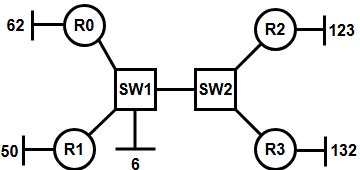
\includegraphics[width=0.4\textwidth]{p4_q1_topology.png}
\end{center}

\textbf{Accounting for Router Interfaces:}
\begin{itemize}
    \item R3 LAN: 132 hosts + 1 gateway = \textbf{133 IP addresses}.
    \item R2 LAN: 123 hosts + 1 gateway = \textbf{124 IP addresses}.
    \item R0 LAN: 62 hosts + 1 gateway = \textbf{63 IP addresses}.
    \item R1 LAN: 50 hosts + 1 gateway = \textbf{51 IP addresses}.
    \item Switched Core (SW1--SW2): 6 hosts + 4 router interfaces (R0, R1, R2, R3) = \textbf{10 IP addresses}.
\end{itemize}

\textbf{Allocation in Descending Order:}
\begin{enumerate}
    \item \textbf{R3 LAN (Needs 133):}
    \begin{itemize}
        \item $2^h - 2 \ge 133 \implies h = 8$ bits ($2^8 - 2 = 254$). Prefix: $/24$ (\texttt{255.255.255.0}).
        \item \textbf{Subnet Address:} \texttt{69.0.0.0/24} (Range: \texttt{69.0.0.1} -- \texttt{69.0.0.254}; Broadcast: \texttt{69.0.0.255})
    \end{itemize}
    \item \textbf{R2 LAN (Needs 124):}
    \begin{itemize}
        \item $2^h - 2 \ge 124 \implies h = 7$ bits ($2^7 - 2 = 126$). Prefix: $/25$ (\texttt{255.255.255.128}).
        \item \textbf{Subnet Address:} \texttt{69.0.1.0/25} (Range: \texttt{69.0.1.1} -- \texttt{69.0.1.126}; Broadcast: \texttt{69.0.1.127})
    \end{itemize}
    \item \textbf{R0 LAN (Needs 63):}
    \begin{itemize}
        \item $2^h - 2 \ge 63 \implies h = 7$ bits ($2^6 - 2 = 62 < 63 \implies h = 7$). Prefix: $/25$ (\texttt{255.255.255.128}).
        \item \textbf{Subnet Address:} \texttt{69.0.1.128/25} (Range: \texttt{69.0.1.129} -- \texttt{69.0.1.254}; Broadcast: \texttt{69.0.1.255})
    \end{itemize}
    \item \textbf{R1 LAN (Needs 51):}
    \begin{itemize}
        \item $2^h - 2 \ge 51 \implies h = 6$ bits ($2^6 - 2 = 62$). Prefix: $/26$ (\texttt{255.255.255.192}).
        \item \textbf{Subnet Address:} \texttt{69.0.2.0/26} (Range: \texttt{69.0.2.1} -- \texttt{69.0.2.62}; Broadcast: \texttt{69.0.2.63})
    \end{itemize}
    \item \textbf{Switched Core Network (Needs 10):}
    \begin{itemize}
        \item $2^h - 2 \ge 10 \implies h = 4$ bits ($2^4 - 2 = 14$). Prefix: $/28$ (\texttt{255.255.255.240}).
        \item \textbf{Subnet Address:} \texttt{69.0.2.64/28} (Range: \texttt{69.0.2.65} -- \texttt{69.0.2.78}; Broadcast: \texttt{69.0.2.79})
    \end{itemize}
\end{enumerate}

\vspace{0.2cm}
\textbf{IV. For the switched network, how many addresses are we wasting? [2 Marks]}
\begin{itemize}
    \item Allocated $/28$ provides $2^4 - 2 = 14$ usable host addresses.
    \item Actually utilized: 6 hosts + 4 router interfaces = 10 addresses.
    \item \textbf{Wasted Usable Addresses:} $14 - 10 = \mathbf{4\text{ usable addresses}}$ (or $16 - 10 = 6$ total block addresses including network and broadcast).
\end{itemize}

\newpage
% =========================================================================
% QUESTION 2
% =========================================================================
\questionheader{Question 2: IPv4 Fragmentation Header \& Datagram Reconstruction}{CO2, CO3}{4 + 3 + 2 = 9}

\textbf{Given Fragment Table:}
\begin{center}
\begin{tabular}{|c|c|c|c|c|}
\hline
\textbf{\#} & \textbf{Total Length} & \textbf{MF} & \textbf{DF} & \textbf{Offset} \\
\hline
10 & 1544 & 1 & 1 & 1692 \\
\dots & \dots & \dots & \dots & \dots \\
15 & 69 & 0 & 1 & 2632 \\
\hline
\end{tabular}
\end{center}

\textbf{I. Identify the header size of the fragment. [4 Marks]}

\textbf{Solution:}
\begin{itemize}
    \item From the course networking study notes, the Fragment Offset for the $k$-th fragment is given by:
    \[
    \text{Fragment Offset}_k = \frac{(k - 1) \times \text{Payload}}{8}
    \]
    where $k$ is the fragment index ($k = 1, 2, 3, \dots$) and $\text{Payload}$ is the data payload size per full fragment.
    \item For Fragment 10 ($k = 10$), the given fragment offset is $\text{Offset}_{10} = 1692$. Applying the formula:
    \[
    1692 = \frac{(10 - 1) \times \text{Payload}}{8} = \frac{9 \times \text{Payload}}{8}
    \]
    \item Solving directly for $\text{Payload}$:
    \[
    \text{Payload} = \frac{1692 \times 8}{9} = \frac{13,536}{9} = \mathbf{1504\text{ bytes}}
    \]
    \item (Cross-check with Fragment 15 ($k = 15$): $\text{Offset}_{15} = \frac{(15 - 1) \times 1504}{8} = \frac{14 \times 1504}{8} = 14 \times 188 = 2632$, matching the table exactly!)
    \item Given Total Length of Fragment 10 is 1544 bytes, the header size is:
    \[
    \text{Header Size} = \text{Total Length} - \text{Payload} = 1544 - 1504 = \mathbf{40\text{ bytes}}
    \]
\end{itemize}
\textbf{Answer:} \textbf{40 bytes} (20-byte base IPv4 header + 20-byte IP options).

\vspace{0.2cm}
\textbf{II. Identify the packet size of the original datagram. [3 Marks]}

\textbf{Solution:}
\begin{itemize}
    \item Fragment 15 has Total Length = 69 bytes. With a 40-byte header, its data payload is:
    \[
    \text{Data in Fragment 15} = 69 - 40 = 29\text{ bytes}
    \]
    \item Total original payload data $= 21,056 + 29 = 21,085$ bytes.
    \item Total size of the original datagram:
    \[
    \text{Original Packet Size} = 21,085 + 40 = \mathbf{21,125\text{ bytes}}
    \]
\end{itemize}
\textbf{Answer:} \textbf{21,125 bytes}.

\vspace{0.2cm}
\textbf{III. Which two fields are required to orderly reassemble the fragmented packets? [2 Marks]}
\begin{enumerate}
    \item \textbf{Identification (ID) Field:} Associates all fragments belonging to the same datagram.
    \item \textbf{Fragment Offset Field:} Determines the exact sequential position of each fragment's payload.
\end{enumerate}

\newpage
% =========================================================================
% QUESTION 3
% =========================================================================
\questionheader{Question 3: Static Routing Configurations \& Administrative Distance}{CO2, CO3}{3 $\times$ 5 = 15}

\begin{center}
    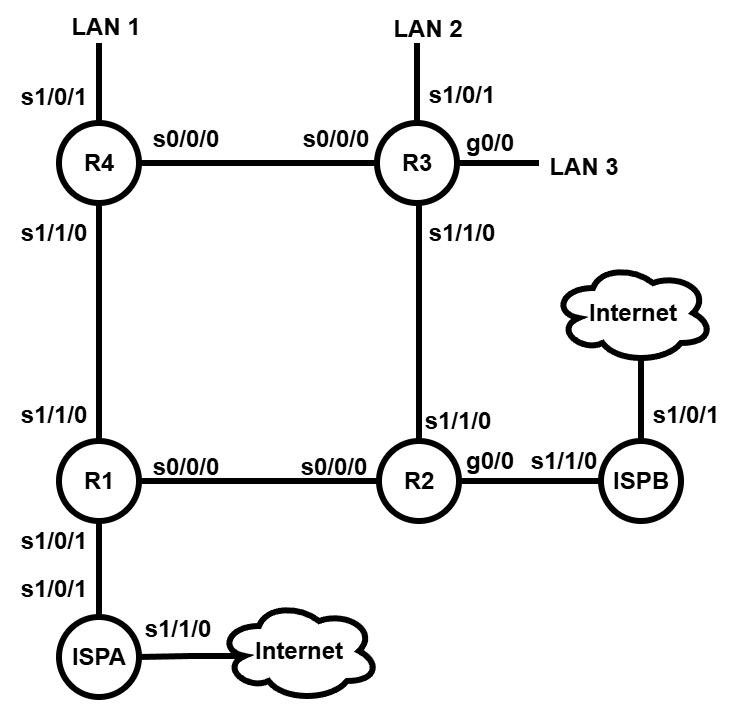
\includegraphics[width=0.4\textwidth]{p4_q3_topology.png}
    \quad
    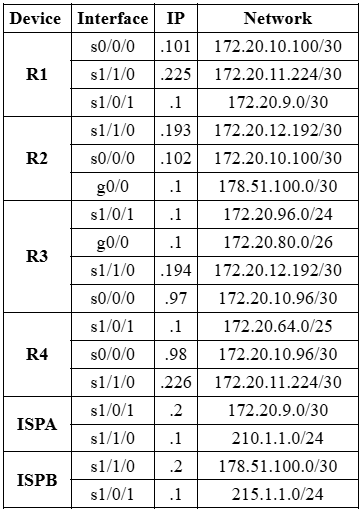
\includegraphics[width=0.45\textwidth]{p4_q3_table.png}
\end{center}

\textbf{I. On R2, add a recursive static route to LAN1 via R1. [3 Marks]}
\begin{itemize}
    \item Destination: LAN1 = \texttt{172.20.64.0/25} (Subnet Mask: \texttt{255.255.255.128}).
    \item Recursive static route specifies the next-hop IP on R1: \texttt{172.20.10.101}.
    \item \textbf{Command:} \texttt{R2(config)\# ip route 172.20.64.0 255.255.255.128 172.20.10.101}
\end{itemize}

\textbf{II. Configure a backup route (directly attached) of the above static route (AD 6). [3 Marks]}
\begin{itemize}
    \item Backup path to LAN1 goes through R3 via interface \texttt{s1/1/0}.
    \item Directly attached specifies the exit interface with $AD = 6$.
    \item \textbf{Command:} \texttt{R2(config)\# ip route 172.20.64.0 255.255.255.128 s1/1/0 6}
\end{itemize}

\textbf{III. On R4, add a recursive default static route to go through the ISPB link. [3 Marks]}
\begin{itemize}
    \item Default route: \texttt{0.0.0.0 0.0.0.0}. Next-hop IP on R3 is \texttt{172.20.10.97}.
    \item \textbf{Command:} \texttt{R4(config)\# ip route 0.0.0.0 0.0.0.0 172.20.10.97}
\end{itemize}

\textbf{IV. If the above route wasn't configured on R4, what problem would have arisen? [3 Marks]}
\begin{itemize}
    \item R4 would have no route for unknown Internet destinations. Traffic from LAN1 destined for the Internet would have no match in R4's routing table, causing R4 to drop the packets and return ICMP Destination Unreachable errors.
\end{itemize}

\textbf{V. Two static routes configured on R3: Which entry should be in R3's table and why? [3 Marks]}
\begin{itemize}
    \item \textbf{Selected Entry:} \textbf{\texttt{S 172.20.64.0/25 [20/0] via 172.20.12.193}}
    \item \textbf{Reason:} When multiple routes exist for the exact same destination prefix, the router selects the route with the \textbf{lowest Administrative Distance (AD)}. The route via \texttt{172.20.12.193} has an AD of 20, which is preferred over the route with AD 30.
\end{itemize}

\newpage
\sectionbanner{SECTION B: ANY TWO OUT OF THREE (12 MARKS)}
\textit{(All questions solved below for complete coverage)}

% =========================================================================
% QUESTION 4
% =========================================================================
\questionheader{Question 4: Distance Vector Convergence \& Failure Advertisement}{CO3}{2 + 4 = 6}

\textbf{I. Networks present in R4's routing table at cold start ($t=0$): [2 Marks]}
Only its directly connected networks:
\begin{enumerate}
    \item LAN1: \texttt{172.20.64.0/25} (connected to \texttt{s1/0/1})
    \item Link R4--R3: \texttt{172.20.10.96/30} (connected to \texttt{s0/0/0})
    \item Link R4--R1: \texttt{172.20.11.224/30} (connected to \texttt{s1/1/0})
\end{enumerate}

\textbf{II. Failure of R3--R2 link and advertisement by R3: [4 Marks]}
\begin{itemize}
    \item \textbf{Information Shared:} R3 advertises that the route to ISPB via R2 is either unreachable (metric $\infty = 16$) or advertises its newly computed path through R4 with an updated metric.
    \item \textbf{Interfaces Advertised To:} R3 transmits this routing update across interface \textbf{\texttt{s0/0/0}} towards Router R4.
\end{itemize}

% =========================================================================
% QUESTION 5
% =========================================================================
\questionheader{Question 5: IPv6 Compression \& All-Nodes Multicast}{CO3}{1 + 1 + 1 + 3 = 6}

\textbf{I. Address Simplification:}
\begin{itemize}
    \item A. \texttt{2001:0db8:12af:0000:0000:0000:0a20:0004} $\to$ \textbf{\texttt{2001:db8:12af::a20:4}}
    \item B. \texttt{0000:0000:0000:0000:0000:0000:0000:0001} $\to$ \textbf{\texttt{::1}}
    \item C. Type of address for (B): \textbf{Loopback Address}.
\end{itemize}

\textbf{II. Sending to all devices on the network in IPv6 without broadcast: [3 Marks]}
\begin{itemize}
    \item IPv6 replaces traditional broadcast with the \textbf{All-Nodes Link-Local Multicast Address}:
    \[
    \mathbf{FF02::1}
    \]
    \item Every IPv6-enabled host on the local link automatically joins the \texttt{FF02::1} multicast group. When a device needs to reach all nodes on the link (e.g., in Neighbor Discovery), it transmits the packet to destination \texttt{FF02::1}.
\end{itemize}

% =========================================================================
% QUESTION 6
% =========================================================================
\questionheader{Question 6: Multi-Switch Broadcast Flooding \& Switch Table Learning}{CO2}{3 + 3 = 6}

\begin{center}
    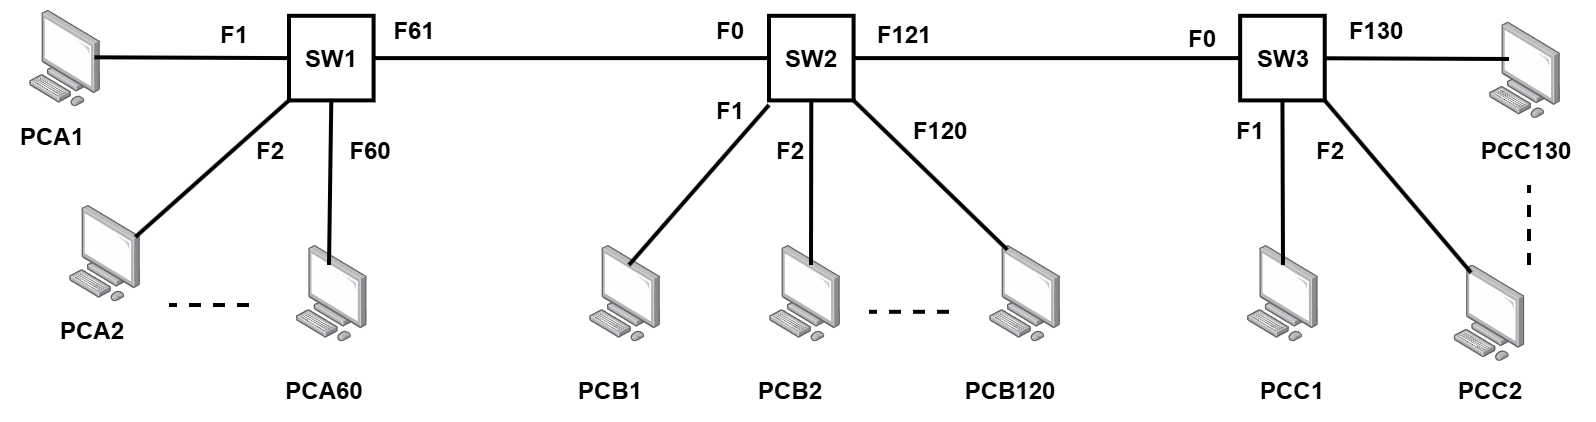
\includegraphics[width=0.85\textwidth]{p4_q6_topology.png}
\end{center}

\textbf{I. How many PCs will receive the ARP request frame? Why? [3 Marks]}
\begin{itemize}
    \item PCA1 broadcasts an ARP request for PCC2. Broadcast frames are flooded out of every active switch port across all connected switches (SW1, SW2, SW3).
    \item \textbf{PCs Receiving the Frame:}
    \begin{itemize}
        \item On SW1: 60 PCs total $- 1$ (the sender PCA1) = 59 PCs.
        \item On SW2: All 120 PCs (PCB1 to PCB120).
        \item On SW3: All 130 PCs (PCC1 to PCC130).
    \end{itemize}
    \item \textbf{Total PCs receiving the request:} $59 + 120 + 130 = \mathbf{309\text{ PCs}}$.
\end{itemize}

\textbf{II. Switch Tables After PCA1 Receives the Reply: [3 Marks]}

\begin{center}
\begin{tabular}{|l|c|}
\multicolumn{2}{c}{\textbf{Switch SW1}} \\
\hline
\textbf{Device} & \textbf{Port} \\
\hline
PCA1 & \texttt{F1} \\
PCC2 & \texttt{F61} \\
\hline
\end{tabular}
\quad
\begin{tabular}{|l|c|}
\multicolumn{2}{c}{\textbf{Switch SW2}} \\
\hline
\textbf{Device} & \textbf{Port} \\
\hline
PCA1 & \texttt{F0} \\
PCC2 & \texttt{F121} \\
\hline
\end{tabular}
\quad
\begin{tabular}{|l|c|}
\multicolumn{2}{c}{\textbf{Switch SW3}} \\
\hline
\textbf{Device} & \textbf{Port} \\
\hline
PCA1 & \texttt{F0} \\
PCC2 & \texttt{F2} \\
\hline
\end{tabular}
\end{center}

\newpage
\sectionbanner{SECTION C: ANY THREE OUT OF FIVE (18 MARKS)}
\textit{(All questions solved below for complete coverage)}

% =========================================================================
% QUESTION 7
% =========================================================================
\questionheader{Question 7: IPv4 Design Fundamentals}{CO2, CO3}{2 + 2 + 2 = 6}

\textbf{I. Why Fragment Offset is measured in multiples of 8 bytes: [2 Marks]}
The Fragment Offset field is only 13 bits wide. Since an IPv4 datagram can be up to $2^{16} - 1 = 65,535$ bytes long, scaling by 8 allows $2^{13} \times 8 = 65,536$ bytes to be indexed within a compact 13-bit header field.

\textbf{II. Why IPv4 is unreliable: [2 Marks]}
IPv4 provides ``best-effort'' delivery without built-in acknowledgments, flow control, or retransmission mechanisms. If a packet encounters congestion or checksum corruption, it is dropped silently. Reliability is delegated to Layer 4 (TCP).

\textbf{III. Scenarios where Traceroute helps more than PING: [2 Marks]}
PING only confirms whether a destination is reachable. Traceroute identifies the exact intermediate hop where a failure, excessive latency, or routing loop occurs.

% =========================================================================
% QUESTION 8
% =========================================================================
\questionheader{Question 8: Centralized DHCP \& DHCP Relay Agent}{CO2}{3 + 3 = 6}

\textbf{I. Why branch PCs cannot obtain IP addresses: [3 Marks]}
DHCPDISCOVER is a broadcast packet. Routers terminate broadcast domains and do not forward broadcast packets across WAN links to headquarters.

\textbf{II. Role of the branch router in solving this issue: [3 Marks]}
Configure the branch router interface as a \textbf{DHCP Relay Agent} (\texttt{ip helper-address <HQ\_DHCP\_IP>}), which intercepts local broadcast discoveries, encapsulates them into unicast UDP packets, and forwards them across the WAN to the headquarters DHCP server.

% =========================================================================
% QUESTION 9
% =========================================================================
\questionheader{Question 9: Carrier-Grade NAT (CGNAT) \& Port Forwarding}{CO2}{3 + 3 = 6}

\textbf{I. Why friends cannot connect to your gaming server: [3 Marks]}
The public IP is shared among multiple customers via **Carrier-Grade NAT (CGNAT)**. The ISP router only tracks outbound sessions; unsolicited inbound connections from the Internet have no matching state entry in the ISP's NAT table and are dropped.

\textbf{II. Networking solution to allow direct reachability: [3 Marks]}
Acquire a **Dedicated Static Public IP address** from the ISP, or configure **Port Forwarding**, or use an encrypted reverse tunnel (e.g., Cloudflare Tunnel / VPN).

% =========================================================================
% QUESTION 10
% =========================================================================
\questionheader{Question 10: IPv6 Encapsulation \& Overhead}{CO2}{4 + 2 = 6}

\textbf{I. IPv6 Tunneling across IPv4: [4 Marks]}
IPv6 packets are encapsulated inside IPv4 packets at the edge router, allowing them to traverse IPv4-only core networks without modifying intermediate routers. This enables cost-effective, incremental transition to IPv6.

\textbf{II. Problems with repeated encapsulation/decapsulation: [2 Marks]}
Adds header overhead (reducing effective payload MTU), increases risk of packet fragmentation, and adds CPU processing delay at tunnel endpoints.

% =========================================================================
% QUESTION 11
% =========================================================================
\questionheader{Question 11: Switch MAC Aging Timer \& Port Migration}{CO2}{3 + 3 = 6}

\textbf{I. Why the PC couldn't print immediately: [3 Marks]}
The switch MAC address table cached the printer's MAC address on the old port. Until the **MAC Aging Timer** (typically 300 seconds / 5 minutes) expired, the switch continued forwarding print frames to the old port.

\textbf{II. What could have been done to enable immediate printing: [3 Marks]}
Manually clear the switch MAC table (\texttt{clear mac address-table dynamic}), or trigger an immediate frame transmission (such as a Gratuitous ARP or ping) from the printer so the switch instantly learns the new port.

\begin{center}
    \rule{\textwidth}{0.8pt}\\[3pt]
    \textbf{\textcolor{primary}{--- END OF EXAMINATION SOLUTION ---}}
\end{center}

\end{document}
